\documentclass[10pt,twocolumn,letterpaper]{article}

\usepackage{cvpr}
\usepackage{times}
\usepackage{epsfig}
\usepackage{graphicx}
\usepackage{amsmath}
\usepackage{amssymb}

% Include other packages here, before hyperref.

% If you comment hyperref and then uncomment it, you should delete
% egpaper.aux before re-running latex.  (Or just hit 'q' on the first latex
% run, let it finish, and you should be clear).
\usepackage[pagebackref=true,breaklinks=true,letterpaper=true,colorlinks,bookmarks=false]{hyperref}


\cvprfinalcopy % *** Uncomment this line for the final submission

\def\cvprPaperID{591} % *** Enter the CVPR Paper ID here
\def\httilde{\mbox{\tt\raisebox{-.5ex}{\symbol{126}}}}

% Pages are numbered in submission mode, and unnumbered in camera-ready
\ifcvprfinal\pagestyle{empty}\fi
\begin{document}

%%%%%%%%% TITLE
\title{Body Signature Recognition\\
{\small NYU-TR-2008-915}}


\author{George Williams
\hspace{0.2in}
Christoph Bregler\thanks{Contact author: chris.bregler@nyu.edu} 
\hspace{0.2in}
Peggy Hackney\\
\and
Sally Rosenthal
\hspace{0.2in}
Ian McDowall 
\hspace{0.2in}
Kirill Smolskiy\\
{\small \url{http://movement.nyu.edu/GreenDotProject}} }




\maketitle
% \thispagestyle{empty}

%%%%%%%%% ABSTRACT
\begin{abstract}
This paper describes a new visual representation of motion that is used to learn and classify body language - what we call ``body signatures'' - of people while they are talking.  We applied this technique to several hours of internet videos and television broadcasts that include US politicians and leaders from Germany, France, Iran, Russia, Pakistan, and India, and public figures such as the Pope, as well as numerous talk show hosts and comedians.  Dependent on the complexity of the task, we show up to 80\% recognition performance and clustering into broader body language categories.
\end{abstract}

%%%%%%%%% BODY TEXT
\section{Introduction}


Global news bombards our senses with world leaders talking about their current policies, problems, and proposed solutions. Most viewers fantasize that they value/don't value what the leaders are saying because of the words that are being used and the face that they see. However, experts in the field of communication agree that up to 80\% of communication is contained in non-verbal �body language.� The movement or what might be called �body signature� determines a major part of the message and the recognition. Talk show hosts and political comedians often capitalize on this phenomenon by actively using their own heightened sense of body movement to bring this aspect to consciousness for the viewers.
 
As human beings we make important decisions, such as whom to vote for, whom to work with, whom to marry, etc., by attuning to these body messages. Therefore, it is important as scientists to understand body movement more fully and include it in our recognition technology.
 
The whole body sends important signals. These signals come from the eyes, eyebrows, lips, head, arms, and torso�all in phrased highly orchestrated movements. In this project, we study how to process these additional signals, the sum of which we call the "body signature."  We hypothesize that every person has a unique body signature, which we are able to detect with statistical classification techniques.  In this paper we study 22 different people of various different international backgrounds while giving speeches.   The data is over 3 hours of video, downloaded from the web, and recorded from broadcast television.  Among others, it includes US politicians, the leaders from Germany, France, Iran, Russia, Pakistan, India, the Pope, and numerous talk show hosts and comedians.
 
\begin{figure}[bt]
\centering
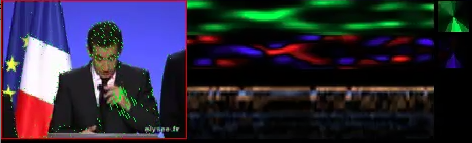
\includegraphics[width=0.96\columnwidth]{Sarkozy_MOS}
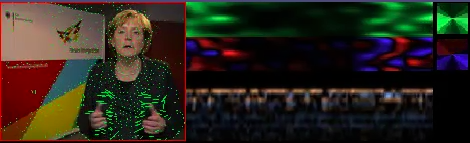
\includegraphics[width=0.96\columnwidth]{Merkel_MOS}
%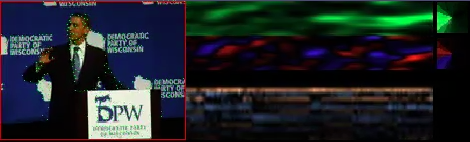
\includegraphics[width=0.96\columnwidth]{Obama_MOS}
%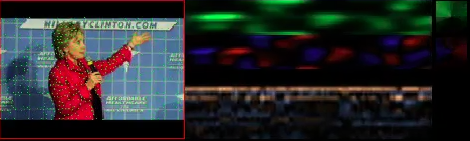
\includegraphics[width=0.96\columnwidth]{Hillary_MOS}
\caption{\label{fig_example_mos} Examples of Motion Signatures.  The green colored signature shows how the orientation of the sparse flow features changes over time (top row), and the red-blue color coded signature shows the delta features (middle row).}
\end{figure}

We present a new video-based feature extraction technique and several methods to train statistical models and classify body signatures.  The recognition architecture is inspired by recent progress in speaker recognition research.  Compared to acoustic speech, the body signature is much more ambiguous, because the body has many parts moving 
either simultaneously or successively. It is like a whole orchestra--not just a single instrument.  Despite this more challenging task, we show up to 80\% recognition performance on various tasks with up to 22 different possible candidates.  We envision this system to be a part of a bigger system that also uses other biometrical techniques such as face-recognition, acoustics, and other modalities.  
 
This paper has 2 main contributions: 1) a new visual feature estimation technique,  based on sparse flow computations and motion angle histograms that we call  �Motion Orientation Signatures� (MOS).  2) Integration of this new feature into a 3-stage recognition system (Gaussian Mixture Models, Super-Features, and SVMs).



\begin{figure}[bt]
\centering
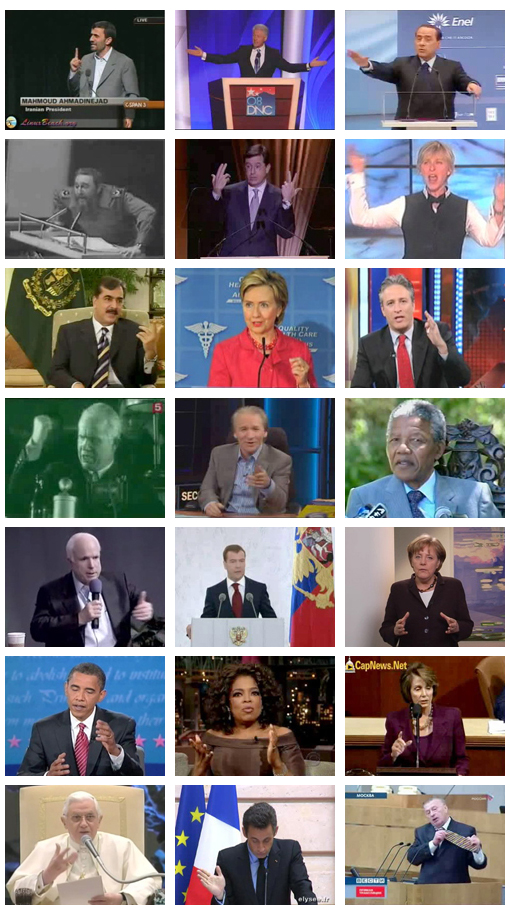
\includegraphics[width=0.96\columnwidth]{matrix}
\caption{\label{fig_examples} Example video frames from our database of over 3 hours of public speeches.
}
\end{figure}


%-------------------------------------------------------------------------
\section{Related Work}
\label{sec_related}

\subsection{People Tracking}
Tracking visual features on people in videos is very difficult.  It is easy to find and track the face because it has clearly defined features, but hands and clothes in standard video are very noisy.   Self-occlusion, drastic appearance change, low resolution (i.e. the hand is sometimes just a few pixels in size), and background clutter make the task of tracking very challenging.  The most impressive people tracking recently has been demonstrated by \cite{ramanan2005spt}. It recognizes body parts in each frame by probabilistic fitting kinematic color and shape models to the entire body.  Many other related techniques have been proposed, but an extensive literature review is beyond the scope of this paper. Please see the survey article by \cite{forsyth2005csh}.  Tracking explicitly body parts would be of great advantage for our problem, but given the low-resolution web footage, it might be impossible to explicitly track the hands this way. Our technique builds on the observation that it is easy to track just a few reliable features for a few frames (instead of tracking body parts over the entire video).   Given those short-term features at arbitrary �unknown� locations, we apply an implicit feature representation that is inspired by techniques that compute global orientation statistics of local features.  Examples include \cite{Freeman95orientationhistograms,Bregler97learningappearance,lowe2004dif,zelnikmanor2006sad,Dalal06humandetection}.

\subsection{Speech and Gesture Recognition}
Our work is also inspired by recent trends in acoustic speaker recognition.  This is a similar task to what we like to perform on the video data.   An excellent survey is published by \cite{muller2007sci}.  Acoustic speech as visual body language depends on many factors, including cultural background, emotional state, and what is being said.  In the acoustic speaker recognition community, many approaches have been proposed.  The simplest techniques apply Gaussian Mixture Models to speech features \cite{reynolds2000svu}, and the most complex models apply a complete low-level phoneme classifier to high-level language model based recognition system \cite{muller2007sci}. Current state-of-the art results are reported  using Support-Vector-Machines applied to various different features \cite{stolcke2005mtf} and \cite{Campbell06supportvector}.  Our classification system is similar to \cite{Campbell06supportvector} in using so called GMM-Super-Vectors.  We will explain these techniques in more detail in section \ref{sec_superfeat} and \ref{sec_svm}. 
In the computer vision community many techniques have been proposed to recognize action, gait, and gesture categories.  Again we refer to \cite{forsyth2005csh} for a survey.

%-------------------------------------------------------------------------
\section{Visual Feature Extraction: Motion Orientation Signatures}

As mentioned in section \ref{sec_related}, we are interested in a robust feature detector that does not use explicit tracking or body part localization (because these techniques will fail frequently, especially on low-res TV and web footage).  We are interested in a feature extraction process that is always able to report a feature vector, no matter how complex the input video is.

\subsection{MOS: Motion Orientation Signatures}

The first step in our extraction schema is the flow computation at such reliable feature locations.  We detect reliable features with the �Good Features� technique by \cite{ST94} and then compute the flow vector with a standard pyramidal Lucas \& Kanade estimation \cite{bouget:pil,lucas1981iir}.  Given these flow estimates, we compute a weighted angle histogram:  The flow directions are discretized into N angle bins (we had good experience with N=9, other choices produced lower recognition performance). Each angle bin then contains the sum of the flow magnitudes in this direction, i.e. large motions have a larger impact than small motions.  We clip flow magnitudes larger than a certain maximum value before adding it to the angle bin.  This makes the angle histogram more robust to outliers.   We then normalize all bin values in dividing them by the number of total features.  This factors out fluctuations caused by a different number of features found in different video frames.   The bin values are then blurred across angle bins and across time with a Gaussian kernel (sigma=1 for angles, and sigma=2 for time).  This avoids aliasing effects in the angle discretization and across time.  (Many web-videos only have 15 fps, some videos are with 24 fps and up-sampled to 30 fps.)  After the spatio-temporal blurring, we further normalize the histogram values to 0-1 over a temporal window (currently t=10).   This factors out video resolution, camera zoom and body size (double resolution creates double flow magnitudes), but could also factor out important features.  Some people's motion signature is based on subtle motions, while others� large movements are much more part of their signature.   For this reason, we keep the normalization constant as one extra feature.  This is inspired by established acoustic front-ends for speech recognition.  The speech features are usually normalized to factor out microphone characteristics, etc., but an �energy� feature is retained.
As with acoustic speech features, we also compute �delta-features�, the temporal derivative of each orientation bin value.    Since the bin values are statistics of the visual velocity (flow), the delta-features cover acceleration and deceleration.  For example if a subject would clap her hands very fast, it would produce large values in the bin values that cover $90^{O}$ and $270^{O}$ (left and right motion), but also large values in the corresponding delta-features.  If a person just circles her hand with constant velocity, the bin values have large values across all angles, but the delta-features have low values.
Figure \ref{fig_example_mos} shows a few examples that demonstrate what signatures are created with certain video input.  The reader is strongly encouraged to watch our video to see the motion signatures.

One very important aspect of this feature representation is that it is invariant to the location of the person.  Given that the flow vectors are computed only at reliable locations, and we clip large flow vectors, the histograms are also very robust to noise.

\subsection{Coarse Locality}

In many videos most of the motion comes from the person who gives the speech, and other background motion is small and �uniformly� distributed, so it has no significant effect on the histogram.  In this case we compute the histograms over the entire video frame.   We also experimented with local region of interests (ROIs) that are either computed on fixed tile areas of a NxM grid, or only focus on the person of interest in running an automatic face detector first. 

\begin{figure}[bt]
\centering
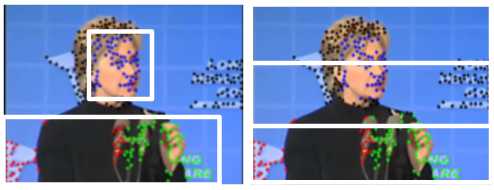
\includegraphics[width=0.96\columnwidth]{hillary_grids}
\caption{\label{fig_roi}\textbf{Left:} Face and Body Tracking, \textbf{Right:} Fixed areas for the motion histogram estimation. }
\end{figure}

\subsubsection{Face and Body Tracking}

There are many mature face-detection algorithms that find with high reliability the location and scale of a face.  We experimented with several methods, and are currently using the Viola-Jones detector \cite{viola2001rod}, but are planning to also use a commercial software package \cite{schneiderman2004odu}. We have also experimented with a full-body detector \cite{Dalal06humandetection} but did not achieve the necessary accuracy. In order to further eliminate false positives and false negatives, we execute following strategy:  When the face detector returns a match, we do not immediately assume that there is a face in that region, since it might be a false positive.   Instead, we confirm the match in that area of the video image by performing the face detection over the next several frames.  Once a face is confirmed in this manner, our technique extrapolates a bounding region (rectangle) around the face large enough to span the typical upright, standing, human body.  At this point,  we confirmed a face region and more importantly a body region in the video frame.  Since we already compute sparse flow on the entire image for our MOS features, we use those features as well to update the location of the face hypothesis.  We compute the average frame-to-frame flow of all flow vectors inside the face region, and update in the next frame the location of the face.  Every 10th frame we run the face-detector again, and confirm that the features haven't drifted too much.  If the face region can not be confirmed by the face-detector after the 10th or the 20th frame, we discard this region This is a more robust strategy, then running the face-detector on each frame, because sometimes the person turns to the side and back frontal, which would make the face-detector fail, but the sparse flow vectors keep track of the face location.  

Despite the advantage of discarding flow features from the background, in only using features that are inside the face location and the derived lower body location, we also have another advantage:  We can compute 2 separate motion histograms, one for the face, and one for the body.  This gives our system a richer feature, instead of having one motion histogram for the entire frame.

The trade-off is,  we still experience many cases where we do not have a successful face detection.  In this case, no MOS features are calculated for those frames.  Despite missing features, the richer features caused on average 4-5\% better recognition performance.

\subsubsection{Static Grid Areas}

Another strategy for computing features that capture some coarse location information, is to compute the motion histograms inside regions that are defined by a static grid.  We experimented with many grid sizes, and got best results with 2 overlapping coarse regions: The top region extends horizontally across the entire frame, and cover the top 2/3 of the frame. The bottom region also covers horizontally the entire frame, and the bottom 2/3 of the frame (Figure \ref{fig_roi} right side).   With this representation we compute 2 motion histograms, and also achieve on average 5\% better recognition performance.   Although the top 2/3 also cover part of the body, and the bottom 2/3 covers part of the face, both histograms together still differ, and the difference between the histograms contains the information of what is different between the head motion and body motion. We currently prefer this representation, since it is not dependent on face-detection failures.  (some subjects had more face-detection failures then others, which put an unwanted bias on our database).  

For all experiments we compute both representations, face-based, and grid-based motion histograms.

\subsection{Other low-level processing}
Our motion histogram normalization partially compensates for camera zoom, but not for camera panes yet.  We are currently experimenting with $2$ alternatives to estimate camera motion: Dominant Motion Estimation, and a heuristic that uses some grid areas at the border of the video frame to estimate background motion.  Once the background motion is estimated, it can be subtracted from all angle histograms.  In this paper we are not using those techniques, and only limit our experiments to static camera recordings.

Furthermore we are also experimenting with different scene cut detection algorithms.  Recording from TV and the web requires scene cut detection, since those videos are usually edited.  In this paper we do not use our current shot detector, and only focus on videos without shot boundaries.

\section{Video Shot Statistics: GMM-Super-Features}
\label{sec_superfeat}
Each video shot is between 5 seconds and 5 minutes long, which equals to a range from 150 time frame shots to 10,000 time frame shots of motion angle histograms features. We separate the shots into a training and an independent test set.  The test set is from recordings at different dates (not different shots from the same video).  For each subject we have videos from 4 to 6 different dates.  Some of them are just a few days apart, some many years apart.  
The training shots are hand labeled with the person�s name (i.e shot X is the Bill Clinton, shot Y is Nancy Pelosi).  We also keep around a lot of unlabeled shots that include other speakers, and both labeled and unlabelled shots are used in a first step to learn biases for our feature representations.  This is again inspired by the acoustic speech community. In the past there have been many different systems proposed, based on convolutional networks, HMMs, Bayesian Networks, and related architectures, but recent experiments in the speech community (like \cite{Campbell06supportvector}) show that Gaussian Mixture Model (GMM) based Super-Features and Support Vector Machines (SVMs) produce state-of-the-art results.  Again, we are inspired by these findings, and also base our shot statistics on GMM-Super-Features and SVMs, although in the future we plan to further investigate more complex architectures.

A Gaussian Mixture Model is first trained on the entire database with the standard EM algorithm.  We experimented with different number of Gaussians, and settled to 16 Gaussians per Mixture Model, which got best recognition performance.  8 and 32 Mixtures produced similar results, but below 8 the recognition performance degraded. In speaker recognition, this is called the Universal Background Model (UBM). Given that UBM model, the statistics of each shot are computed in MAP adapting the GMM to the shot \cite{Campbell06supportvector,gauvain1994mpe}.  This is done with another EM step.  The M step is not completely updating the UBM model, but rather uses a trade-off term on how much the original Gaussian is weighted vs the new result from the M-step.  A GMM-Super-Feature is the difference between the UBM mean vectors and the new MAP adapted mean vectors.  If the shot is similar to the statistics of the UBM, the difference in mean vectors is very small.   If the new shot has some unique motion, then at least one mean vector has a large difference to the UBM model.  The GMM-Super-Feature is a fixed-length vector that describes the statistics of the variable length shot.   We use these vectors now for classification and clustering.



\section{Recognition and Clustering Experiments}
\label{sec_svm}

\subsection{SVM based classification}
\begin{figure}[tb]
\centering
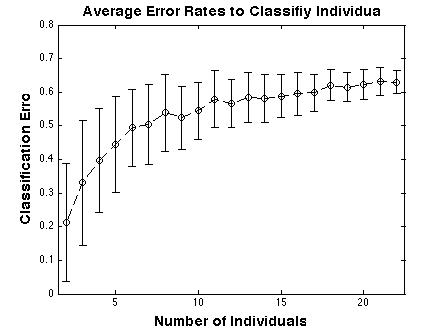
\includegraphics[width=0.96\columnwidth]{sub_err}
\caption{\label{fig_sub_err} 
Average classification errors. Each experiment was repeated 100 times.  At each time, randomly a subset of n subjects were picked from the full pool of 22 possible subjects. Also, the training set and test set was randomly split into equal independent number of videos.
}
\end{figure}

Like in \cite{Campbell06supportvector} we can feed those GMM-Super-Features into a standard SVM classifier, in further scaling the means with the mixing coefficients and covariances of the GMM model:
A linear SVM kernel is a good approximation to the KL-divergence between two utterances.    This is exactly the property that we want to model.   A large distance between the Super-Features of two shots in the SVM hyper plane corresponds to large statistical difference between the shots.
For all our classification experiments we use the multi-class extension of the SVM-light package \cite{joachims:mls}.    

Figure \ref{fig_examples}  shows some example video frames from our database.  In total we have 22 different subjects.  For each subject we have at least 4 different videos, sometimes up to 6 different videos. All were recorded at different times.  Each video was between 5 seconds to 5 minutes.  Our database contains (in alphabetical order): Mahmoud Ahmadinejad, Silvio Berlusconi, Fidel Castro, Bill Clinton, Hillary Clinton, Stephen Colbert, Ellen DeGeneres, Yousaf Gillani, Nikita Khrushchev, Bill Maher, Nelson Mandela, John McCain, Dmitry Medvedev, Angela Merkel, Barack Obama, Nancy Pelosi, Pope Benedict XVI, Nicolas Sarkozy, Manmohan Singh, Jon Stewart, Oprah Winfrey, and Vladimir Volfovich Zhirinovsky.

Figure \ref{fig_sub_err} shows recognition rates using this database. We measured the performance on various subsets.  For instance recognizing one out of two people is much easier then recognizing one out of 22 people. Each classification error in the graph of figure \ref{fig_sub_err} is the average of 100 experiments.  In each experiment we picked randomly the subset of N people, and randomly split the videos into a training set and a test test.  The GMMs, super-features,  and SVMs were first trained on the training set (for each category only 2-3 videos), and then tested on the independent test set.
As you can see, for 2 people classification, we have on average 80\% correct performance, but a much larger variance in performance values.  This is due to the fact that some pairs of subjects are harder to distinguish and might also have less video data than others. For 22 people classification we only get to around 37\% correct.  This might be still valuable as a "weak" features for a multi-modal recognition system.  It is beyond the scope of this paper, but we are currently also evaluating this system in concert with an acoustic speaker recognition system, and our initial experiments have shown an improvement of acoustic speaker recognition rates in including these visual features.    

We also experimented with another task, the classification of broader body language categories.  Several subjects might have very similar body language, and it might be more useful to classify broader categories (that several subjects share.)  

\subsection{Body Language Clustering}
We experimented in applying multi-class spectral clustering \cite{yu2003msc} to our Super-Feature vectors to discover sub groups of subjects with similar body language.   Figure \ref{fig_clusters} shows the distance matrix of all 22 subjects using the Bhattacharya distance \cite{kailath1967dab} between the Super-Vectors (this distance measures a similar metric as the KL-divergence used for the SVM experiments).    We ran the multi-class spectral clustering algorithm for several different number of clusters, and re-trained our SVM for the different cluster categories instead of individual target values.  Figure \ref{fig_cat_err} shows our recognition rates (again the average of 100 random split ups between test and training sets). As you can see, using clusters improved significantly the performance.  For instance we only get 33\% error on a 5 category problem using clusters, instead of 49\% error if we try to distinguish 5 individuals. 

As we mentioned before, we envision this system to be part of a larger multi-modal system that also uses face-recogntion, acoustic speaker verification, and other modalities.  In this context, the recognition rates that we achieve here could be used to further boost other recognition rates from the other modalities.

\begin{figure}[bt]
\centering
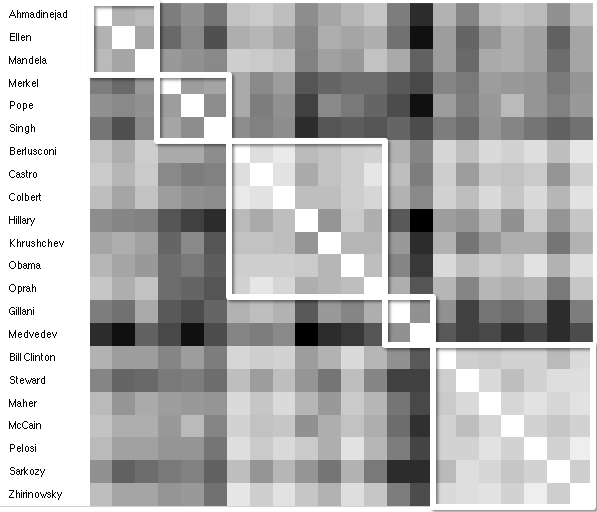
\includegraphics[width=0.96\columnwidth]{cluster_pix}
\caption{\label{fig_clusters} 
Spectral clusters.  The rows and columns are re-ordered such that clustered subjects are in proximity to each other.  White means the subjects are close to each other, and dark means they are further apart from each other.
}
\end{figure}

\begin{figure}[bt]
\centering
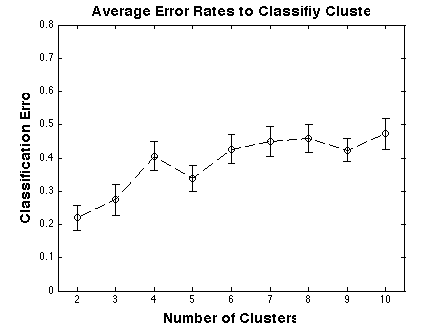
\includegraphics[width=0.96\columnwidth]{cat_err}
\caption{\label{fig_cat_err} 
Average classification errors. Each experiment was repeated 100 times.  At each time, randomly  the training set and test set was randomly split into equal independent number of videos.
}
\end{figure}


\subsection{Sanity-Experiments: Simple Maximum Log-Likelihood Classification}

In order to visualize how the Motion Orientation Histograms and GMM-Super-Features process the different example videos, we also experimented with a simpler classification method:  we computed the log-likelihood of the GMM model for each time-frame.  We accumulated all log-likelihood values over the entire test-shot, and compared the values across  C different GMM models (C is the number of subjects).  This was the standard method used in speaker recognition a decade ago.   We discovered this technique only produces 5\% - 10\% larger error values then the SVM based classification, but allowed us to more quickly visualize how the different likelihoods grow over time while watching the video.
Please see the supplementary video that shows a few examples.   

\section{Discussion and Future Plans}

We demonstrated a simple but effective visual feature extraction schema, the Motion Orientation Signatures, and further mapping of these features into GMM based Super-Vectors and a SVM based classification.   At the time of writing this paper, we had a collection of 22 subjects, but our database is growing day by day, and we envision to have collected a significant larger database in the coming months.   We showed that on this complex task of body-language detection, we achieve good recognition performance.   While doing this, we ignored many important aspects, like the context of the video, what emotional state the speaker is in, and many other factors that have influence on the body-language.  We also believe these features can be used for many other tasks, like action recognition, or even general video classification (i.e. is this a person, or a car, or another object with a typical motion statistics).    Further research is planned on a richer feature extraction theme, that incorporates spatial information, and also improves the face-detector in considering other features that are in the video.  Besides our experiments with SVM classification, we also plan to apply unsupervised techniques and other supervised methods, like Convolutional Networks and different incarnations of Dynamic Belief Networks on our features.  We expect that these networks can capture more long-range temporal features that are present in the signal. Now that we can teach a computer to watch TV and identify selected individuals based on their body signature, we could imagine a not so distant future project in which un-supervised machine performs a far more complex task: monitoring all TV channels, 24/7, and making increasingly fine distinctions among a barrage of video that would overwhelm the human eye.

\section{Acknowledgements}
We would like to thank Andreas Stolcke for pointing us to the right Speaker Verification Systems, and the Office of Naval Research (ONR N000140710414) and the National Science Foundation (NSF 0329098, NSF 0325715) for supporting this research.

{\small
\bibliographystyle{ieee}
\bibliography{vision}
}

\end{document}
